\documentclass{article}
\usepackage{import}
\subimport*{../../}{macro}

\setlength\parindent{0px}

\begin{document}
\setcounter{aprob}{0}
\setcounter{bprob}{0}
\title{Homework \#1}
\author{
    \normalsize{CSE 446/546: Machine Learning}\\
    \normalsize{Sami Turbeville}\\
    \normalsize{Collab: Shabab Ahmed}\\
    \normalsize{Due: \textbf{Wednesday} October 20, 2021 11:59pm}\\
    \normalsize{\textbf{A:} 59 points, \textbf{B:} 30 points}
}
\date{{}}
\maketitle

\noindent Please review all homework guidance posted on the website before submitting to GradeScope. Reminders:
\begin{itemize}
    \item Make sure to read the ``What to Submit'' section following each question and include all items.
    \item Please provide succinct answers and supporting reasoning for each question. Similarly, when discussing experimental results, concisely create tables and/or figures when appropriate to organize the experimental results. All explanations, tables, and figures for any particular part of a question must be grouped together.
    \item For every problem involving generating plots, please include the plots as part of your PDF submission.
    \item When submitting to Gradescope, please link each question from the homework in Gradescope to the location of its answer in your homework PDF. Failure to do so may result in deductions of up to \points{5}. For instructions, see \url{https://www.gradescope.com/get_started#student-submission}.
    \item Please recall that B problems, indicated in \boxed{\textrm{boxed text}}, are only graded for 546 students, and that they will be weighted at most 0.2 of your final GPA (see website for details). In Gradescope there is a place to submit solutions to A and B problems separately. You are welcome to create just a single PDF that contains answers to both, submit the same PDF twice, but associate the answers with the individual questions in Gradescope. 
    \item If you collaborate on this homework with others, you must indicate who you worked with on your homework. Failure to do so may result in accusations of plagiarism.
    \item For every problem involving code, please include the code as part of your PDF for the PDF submission \emph{in addition to} submitting your code to the separate assignment on Gradescope created for code. Not submitting all code files will lead to a deduction of \points{1}.  
\end{itemize}

Not adhering to these reminders may result in point deductions. \\

\clearpage{}


% Start of Problems:

\section*{Short Answer and ``True or False'' Conceptual questions}
\begin{aprob}
    The answers to these questions should be answerable without referring to external materials.  Briefly justify your answers with a few words.
    
    \rule{\textwidth}{0.25pt}
    \begin{enumerate}
        \item\points{2} In your own words, describe what bias and variance are? What is bias-variance tradeoff?
        
        Bias arises because we use only a subset of the dataset to train the model so the sample will not be able to capture the true behavior of the set. This can be reduced by resampling (for example k-folding).
        Variance is how much the predicted values differs from some of the data, this can be a subset of the training set or the test set. Variance is reduced as model complexity increases because it is able to predict the set better.
        The bias-variance tradeoff is exactly that, a trade off between high bias and low variance with more complex models and vice versa. So, you have to find the sweet spot where variance and bias are minimized. This is also related to under- and overfitting the model.

        \rule{\textwidth}{0.25pt}
        \newpage
        \item \points{2} What \textbf{typically} happens to bias and variance when the model complexity increases/decreases?

        As complexity increases bias decreases and variance increases, and vice versa. There is a sweet spot somewhere in between where bias is considerably low and variance is also minimized. There will be some unusual cases where this may not be the

        \rule{\textwidth}{0.25pt}
        \newpage
        \item \points{1} True or False: A learning algorithm will always generalize better if we use fewer features to represent our data.

        \textbf{False}, with fewer training data points the model will not generalize as well because it doesn't have as many features to detect and it will be biased towards this training data which may not be the best representation of the complete data.
        As model complexity decreases, bias increases.

        \rule{\textwidth}{0.25pt}
        \newpage
        \item \points{2} True or False: Hyperparameters should be tuned on the test set. Explain your choice and detail a procedure for hyperparameter tuning.

        \textbf{False}, never ever ever use the test set. I would use the k-folding cross validation because it is faster even though it is more biased. 

        For the k-folding cross validation, you devide the training set into $k$ equal parts, $D_1, D_2, \dots, D_k$. Then the estimator error on the classifier $\hat{f}_{D \backslash D_i} (x)$ for each $i$ is 
        $$ \text{error}_{D_i} =  \frac{1}{|{D_i}|} \sum_{(x_j,y_j)\in D_i} (y_i - \hat{f}_{D \backslash D_i} (x_i) )^2 $$
        Then the $k$-folding error is the average of these errors over each $D_i$.
        $$ \text{error}_{k_fold} = \frac{1}{k} \sum_{i=0}^k \text{error}_{D_i} $$
        We find this values for each hyperparameter, $\lambda$, and choose the one with minimal error.

        \rule{\textwidth}{0.25pt}
        \newpage
        \item \points{1} True or False: The training error of a function on the training set provides an overestimate of the true error of that function.

        \textbf{False}, the testing error will be at least as large as the training error. The training set will fit better because the same data (training set) was used to generate the model and calculate the error. The training error is an underestimates of the true error of the function.

        \rule{\textwidth}{0.25pt}
        \newpage
    \end{enumerate}

\end{aprob}

\section*{Maximum Likelihood Estimation (MLE)}

\begin{aprob}
    You're the Reign FC manager, and the team is five games into its 2021 season. The number of goals scored by the team in each game so far are given below:

    \[
      [2, 4, 6, 0, 1].
    \]

    Let's call these scores $x_1, \cdots, x_5$. Based on your (assumed iid) data, you'd like to build a model to understand how many goals the Reign are likely to score in their next game. You decide to model the number of goals scored per game using a \emph{Poisson distribution}. Recall that the Poisson distribution with parameter $\lambda$ assigns every non-negative integer $x = 0, 1, 2, \cdots$ a probability given by
    \[
      \mathrm{Poi}(x | \lambda) = e^{-\lambda} \frac{\lambda ^ x}{x!}.
    \]

    \begin{enumerate}
        \item \points{5} Derive an expression for the maximum-likelihood estimate of the parameter $\lambda$ governing the Poisson distribution in terms of goal counts for the first $n$ games: $x_1, \cdots, x_n$. (Hint: remember that the log of the likelihood has the same maximizer as the likelihood function itself.)

        \item \points{2} Give a numerical estimate of $\lambda$ after the first five games. Given this $\lambda$, what is the probability that the Reign score $6$ goals in their next game?
        \item \points{2} Suppose the Reign score 8 goals in their 6th game. Give an updated numerical estimate of $\lambda$ after six games and compute the probability that the Reign score $6$ goals in their 7th game.
    \end{enumerate}

    \rule{\textwidth}{0.25pt}

    \subsubsection*{Solutions}
    \begin{enumerate}
        \item Let's start by finding the probability of getting this combination of scores $x_1, ... , x_5$
        \begin{align*}
            P(x_1\cdots x_n) &= P(x_1)P(x_2)\cdots P(x_n) & &\text{ since scores are iid} \\
            &= \prod e^{-\lambda}\frac{\lambda^x}{x!} & &\text{ by definition} \\
            ln( P( x_1 \cdots x_n ) ) &= ln( \prod e^{-\lambda}\frac{\lambda^{x_i}}{x_i!} ) & &\text{ taking natural log of both sides}\\
            &= \sum ln( e^\lambda \frac{\lambda^{x_i}}{x_i!} ) & &\text{since log turns product to sum}\\
            &= \sum  -\lambda + x_i ln( \lambda ) - ln( x_i! )  \\
            &= -n \lambda + ln(\lambda) \sum ( x_i ) - \sum( ln(x_i!) ) \\
        \end{align*}
        Then we differentiate to get the maximum.
        \begin{align*}
            \frac{\diff}{\diff \lambda} ln( P( x_1 \cdots x_n ) ) &= \frac{\diff}{\diff \lambda} \lbrack -n \lambda + ln(\lambda) \sum ( x_i ) - \sum( ln(x_i!) ) \rbrack\\
            &= -n + \frac{1}{\lambda} \sum ( x_i )- 0 \\
            0 &= -n + \frac{1}{\lambda} \sum ( x_i ) & & \text{maximized when differential is 0}\\
            n &= \frac{1}{\lambda} \sum ( x_i ) & & \text{solve for }\lambda \\
            \lambda &= \frac{1}{n} \sum ( x_i ) \\
        \end{align*}
        Thus,
        $$ \boxed{\lambda =  \text{mean} (x_i, ... , x_n)} $$
        \rule{\textwidth}{0.25pt}
        \newpage

        \item After the first five games,
        \[ \lambda = \frac{1}{5} (2+4+6+0+1) \]
        $$ \boxed {\lambda = \frac{13}{5} = 2.6 }$$
        The probability that Reign score 6 goals in their next game is
        \begin{align*}
            Poi(x|\lambda) &= e^{-\lambda} \frac{\lambda^x}{x!} \\
            Poi(6|2.6) &= e^{-2.6} \frac{2.6^6}{6!} \\
        \end{align*}
        $$ \boxed { Poi(6|2.6) = 0.0319 } $$
        \rule{\textwidth}{0.25pt}
        \newpage

        \item After the sixth game if Reign scores 8 goals, then
        \[ \lambda = \frac{1}{6} (2+4+6+0+1+8) \]
        $$ \boxed {\lambda = \frac{21}{6} =  3.5}$$
        The probability that Reign score 6 goals in their next game is
        \begin{align*}
            Poi(x|\lambda) &= e^{-\lambda} \frac{\lambda^x}{x!} \\
            Poi(6|3.5) &= e^{-3.5} \frac{3.5^6}{6!} \\
        \end{align*}
        $$ \boxed { Poi(6|3.5) = 0.0770983 } $$
    \end{enumerate}
\end{aprob}

\rule{\textwidth}{0.25pt}
\newpage
\begin{aprob}
    \points{10} \textit{(Optional Background)} In World War 2, the Allies attempted to estimate the total number of tanks the Germans had manufactured by looking at the serial numbers of the German tanks they had destroyed. The idea was that if there were $n$ total tanks with serial numbers $\{1,\cdots,n\}$ then its reasonable to expect the observed serial numbers of the destroyed tanks constituted a uniform random sample (without replacement) from this set. The exact maximum likelihood estimator for this so-called \emph{German tank problem} is non-trivial and quite challenging to work out (try it!). For our homework, we will consider a much easier problem with a similar flavor.\\

    Let $x_1,\cdots,x_n$ be independent, uniformly distributed on the continuous domain $[0,\theta]$ for some $\theta$. What is the Maximum likelihood estimate for $\theta$?
    \subsubsection*{Solution}
    \begin{itemize}
        \item The pdf for the iid on the continuous domain from 0 to $\theta$ is
            \[ f(x_1 \cdots x_n) = \frac{1}{\theta} \]
            for $x_i \in [0,\theta]$. Because they are iid, we can do the following
            \[ f(x_1 \cdots x_n) = f(x_1)f(x_2) \cdots f(x_n) = \frac{1}{\theta^n} \]
            The maximum $\theta$ is found by taking the derivative which we be the same as the derivative of the log.
            \[ ln((\frac{1}{\theta})^n) = -n ln(\theta) \]
            \[ \frac{\diff}{\diff \theta} -n ln(\theta) = -\frac{n}{\theta} \]
            Since $n$ and $\theta$ must be non-negative, then
            \[ -\frac{n}{\theta} \leq 0 \]
            So $\theta$ is maximized for the largest $x_i$. So,
            \[ \boxed{\text{MLE}(\theta) = \text{max}(x_1,...,x_n)} \]
    \end{itemize}
\end{aprob}

\rule{\textwidth}{0.25pt}

\newpage
\section*{Polynomial Regression}
{\bf Relevant Files}\footnote{{\bf Bold text} indicates files or functions that you will need to complete; you should not need to modify any of the other files.}
\vspace{-1.2em}
\begin{multicols}{2}
    \begin{itemize}[noitemsep,nolistsep]
        \item \texttt{\bf polyreg.py}
        \item \texttt{linreg\_closedform.py}
        \item \texttt{test\_polyreg\_univariate.py}
        \item \texttt{test\_polyreg\_learningCurve.py}
        \item \texttt{data/polydata.dat}
    \end{itemize}
\end{multicols}

\begin{aprob}
    \points{10} Recall that polynomial regression learns a function $h_{\bm{\theta}}(x) = \theta_0 + \theta_1 x + \theta_2 x^2 + \ldots + \theta_d x^d$, where $d$ represents the polynomial's highest degree.  We can equivalently write this in the form of a  linear model with $d$ features
    \begin{equation}
        h_{\bm{\theta}}(x) = \theta_0 + \theta_1 \phi_1(x)  + \theta_2 \phi_2(x)  + \ldots + \theta_d \phi_d(x)  \enspace ,
    \end{equation}
    using the basis expansion that $\phi_j(x) = x^j$.  Notice that, with this basis expansion, we obtain a linear model where the features are various powers of the single univariate $x$.  We're still solving a linear regression problem, but are fitting a polynomial function of the input.\\
    
    Implement regularized polynomial regression in \texttt{polyreg.py}.  You may implement it however you like, using gradient descent or a closed-form solution.  However, I would recommend the closed-form solution since the data sets are small; for this reason, we've included an example closed-form implementation of linear regression in \texttt{linreg\_closedform.py} (you are welcome to build upon this implementation, but make CERTAIN you understand it, since you'll need to change several lines of it).  You are also welcome to build upon your implementation from the previous assignment, but you must follow the API below.  Note that all matrices are actually 2D numpy arrays in the implementation.\\
    
    \begin{itemize}[noitemsep, nolistsep]
        \item \texttt{\_\_init\_\_(degree=1, regLambda=1E-8)} : constructor with arguments of $d$ and $\lambda$
        \item \texttt{fit(X,Y)}: method to train the polynomial regression model
        \item \texttt{predict(X)}: method to use the trained polynomial regression model for prediction
        \item \texttt{polyfeatures(X, degree)}: expands the given $n \times 1$ matrix $X$ into an $n \times d$ matrix of polynomial features of degree $d$.  Note that the returned matrix will not include the zero-th power.\\
    \end{itemize}
    
    Note that the \texttt{polyfeatures(X, degree)} function maps the original univariate data into its higher order powers.  Specifically, $X$ will be an $n \times 1$ matrix $(X \in \mathbb{R}^{n \times 1})$ and this function will return the polynomial expansion of this data, a $n \times d$ matrix.  Note that this function will {\bf not} add in the zero-th order feature (i.e., $x_0 = 1$).  You should add the $x_0$ feature separately, outside of this function, before training the model.

    \begin{wrapfigure}{R}{0.42\textwidth}
        \centering
        \vspace{-1em}
        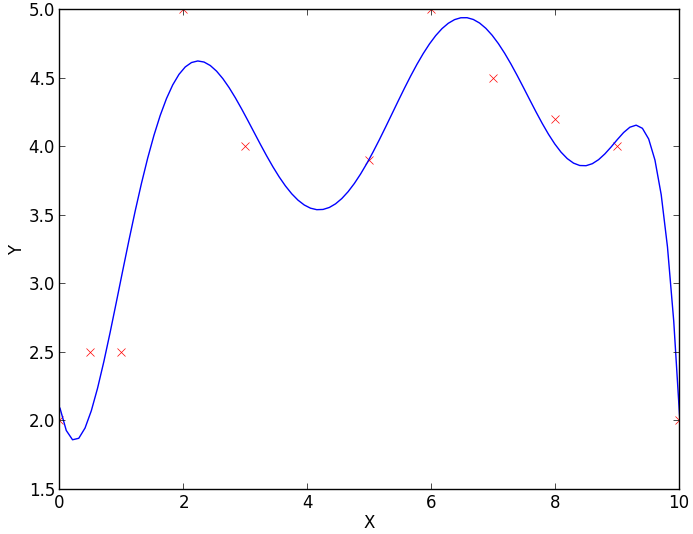
\includegraphics[width=0.4\textwidth]{../img/polyregDegree8.png}
        \vspace{-1em}
        \caption{Fit of polynomial regression with $\lambda = 0$ and $d = 8$}\label{fig:polyregUnivariate}
        \vspace{-2em}
    \end{wrapfigure}

    By not including the $x_0$ column in the matrix \texttt{polyfeatures()}, this allows the \texttt{polyfeatures} function to be more general, so it could be applied to multi-variate data as well. (If it did add the $x_0$ feature, we'd end up with multiple columns of 1's for multivariate data.)\\

    Also, notice that the resulting features will be badly scaled if we use them in raw form.  For example, with a polynomial of degree $d = 8$ and $x = 20$, the basis expansion yields $x^1 = 20$ while $x^8 = 2.56 \times 10^{10}$ -- an
    absolutely huge difference in range.  Consequently, we will need to standardize the data before solving linear regression.  Standardize the data in \texttt{fit()} after you perform the polynomial feature expansion.  You'll need to apply the same standardization transformation in \texttt{predict()} before you apply it to new data.\\

    Run \texttt{test\_polyreg\_univariate.py} to test your implementation, which will plot the learned function.  In this case, the script fits a polynomial of degree $d=8$ with no regularization $\lambda = 0$.  From the plot, we see that the function fits the data well, but will not generalize well to new data points.  Try increasing the amount of regularization, and in 1-2 sentences, describe the resulting effect on the function (you may also provide an additional plot to support your analysis).

    \rule{\textwidth}{0.25pt}

    \subsection*{Solution}

    Figure \ref{fig:poly_ref_d8} shows the polynomial regression with degree 8 and various $\lambda$ values where $\lambda$ is the regularization. As the regularization parameter ($\lambda$) increases, the function supposedly becomes more ``general'' but that is not actually what we want to do here because it is overgeneralizing and just flattening to a horizontal line near $y=k$, a constant. As $\lambda \rightarrow \infty$, the regression becomes linear at $y \approx k$.

    \begin{figure}
        \centering
        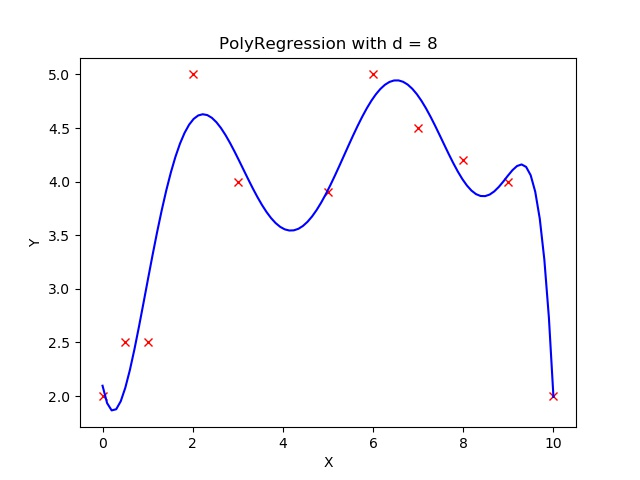
\includegraphics[width=0.5\textwidth]{../../../hw1-code/homeworks/poly_regression/fig1.jpg}
        \caption{Plot of the polynomial regression with degree 8, $\lambda$=0.}\label{fig:poly_reg}
    \end{figure}

    \begin{figure}
        \centering
        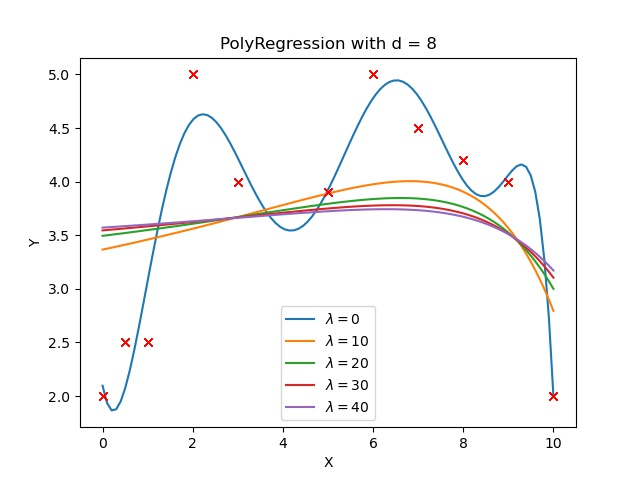
\includegraphics[width=0.5\textwidth]{../../../hw1-code/homeworks/poly_regression/fig2.jpg}
        \caption{Plot of the polynomial regression with degree 8 and various $\lambda$ values. The regularization increases with $\lambda$.} \label{fig:poly_ref_d8}
    \end{figure}

    \begin{figure}
        \centering
        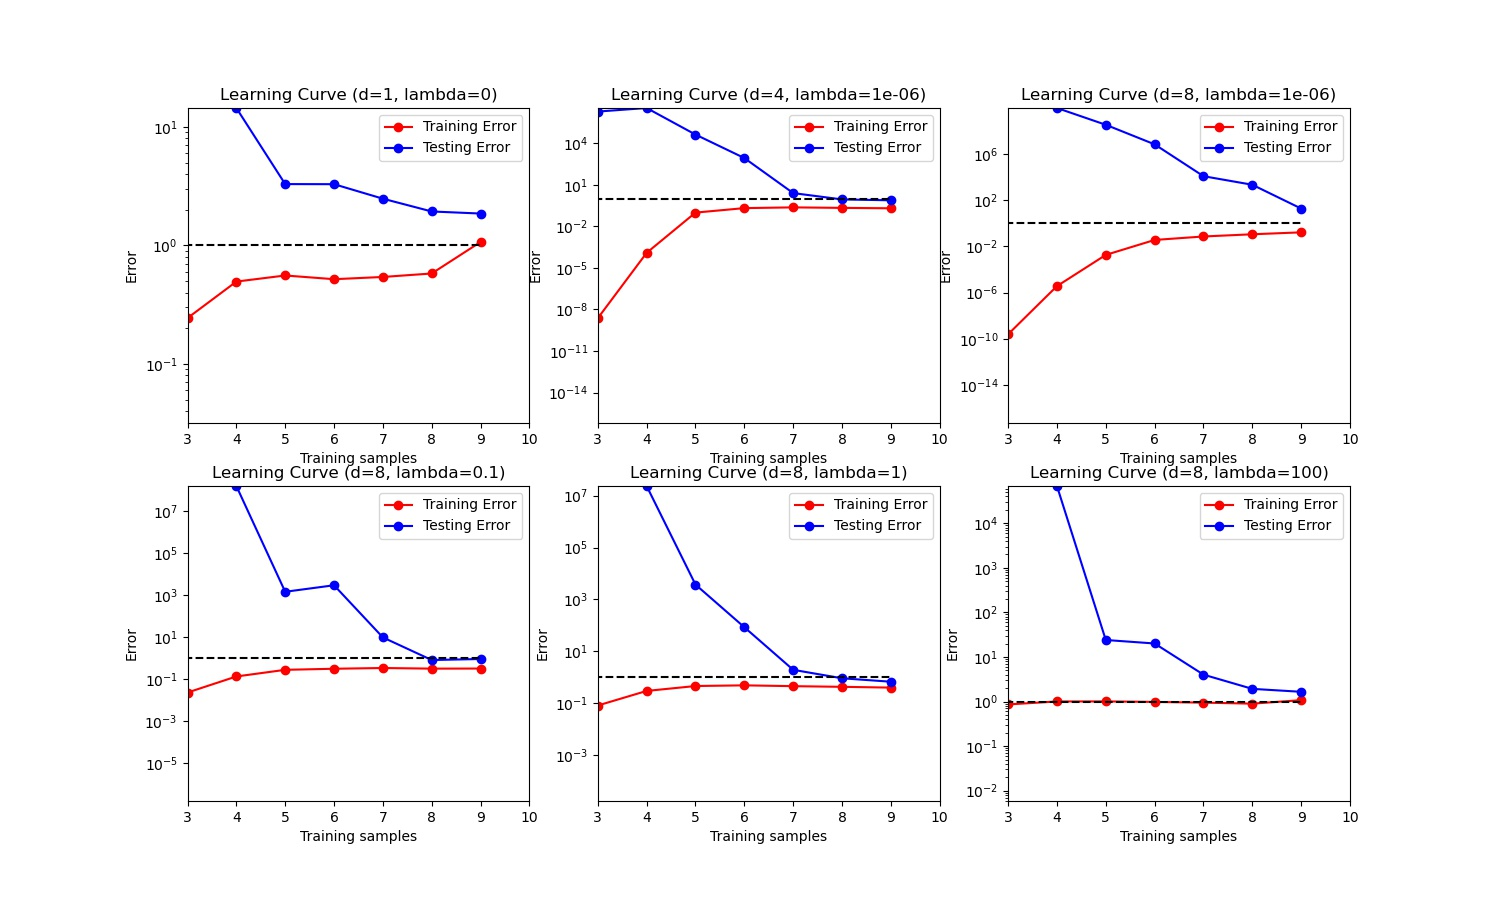
\includegraphics[width=\textwidth]{../../../hw1-code/homeworks/poly_regression/fig3.jpg} \label{fig:mse}
        \caption{Plot of MSE (learning curve) of a trainng set (red) and a test set (blue). The dashed black line denotes the values where error $=1$.}
    \end{figure}

\end{aprob}

\rule{\textwidth}{0.25pt}

\newpage
\section*{Administrative}
\begin{aprob}
\begin{enumerate}
    \item \points{2} About how many hours did you spend on this homework? There is no right or wrong answer :)

    Probably around 5 - 7 hours I did not keep count.
\end{enumerate}

\end{aprob}

\newpage
\section*{Code}

\begin{lstlisting}[language=Python]

    """
    polyreg.py
    Template for polynomial regression
    AUTHOR Eric Eaton, Xiaoxiang Hu
    """

    from typing import Tuple

    import numpy as np

    from utils import problem


    class PolynomialRegression:
        @problem.tag("hw1-A", start_line=5)
        def __init__(self, degree: int = 1, reg_lambda: float = 1e-8):
            """Constructor
            """
            self.degree: int = degree
            self.reg_lambda: float = reg_lambda
            # Fill in with matrix with the correct shape
            self.weight: np.ndarray = None  # type: ignore
            self.mean: np.ndarray = None
            self.std: np.ndarray = None

        @staticmethod
        @problem.tag("hw1-A")
        def polyfeatures(X: np.ndarray, degree: int) -> np.ndarray:
            """
            Expands the given X into an (n, degree) array of polynomial features of degree degree.

            Args:
                X (np.ndarray): Array of shape (n, 1).
                degree (int): Positive integer defining maximum power to include.

            Returns:
                np.ndarray: A (n, degree) numpy array, with each row comprising of
                    X, X * X, X ** 3, ... up to the degree^th power of X.
                    Note that the returned matrix will not include the zero-th power.

            """
            X_ = np.zeros((X.shape[0],degree))
            for i in range(degree):
                X_[:,i] = X[:,0]**(i+1)
            return X_

        @problem.tag("hw1-A")
        def fit(self, X: np.ndarray, y: np.ndarray):
            """
            Trains the model, and saves learned weight in self.weight

            Args:
                X (np.ndarray): Array of shape (n, 1) with observations.
                y (np.ndarray): Array of shape (n, 1) with targets.

            Note:
                You need to apply polynomial expansion and scaling at first.
            """
            # expand the array using polyfeatures()
            X_expanded = self.polyfeatures(X, self.degree)

            # standardize
            self.mean = np.mean(X_expanded, axis=0)
            self.std  = np.std(X_expanded, axis=0)
            n = len(X)
            if n == 1:
                X_standard = X
            else:
                X_standard = (X_expanded - self.mean) / self.std

            # add 1s column
            X_ = np.c_[np.ones([n, 1]), X_standard]

            n, d = X_.shape
            # remove 1 for the extra column of ones we added to get the original num features
            d = d - 1

            # construct reg matrix
            reg_matrix = self.reg_lambda * np.eye(d + 1)
            reg_matrix[0, 0] = 0

            # analytical solution (X'X + regMatrix)^-1 X' y
            self.weight = np.linalg.pinv(X_.T.dot(X_) + reg_matrix).dot(X_.T).dot(y)

        @problem.tag("hw1-A")
        def predict(self, X: np.ndarray) -> np.ndarray:
            """
            Use the trained model to predict values for each instance in X.

            Args:
                X (np.ndarray): Array of shape (n, 1) with observations.

            Returns:
                np.ndarray: Array of shape (n, 1) with predictions.
            """
            n = len(X)
            # expand the array using polyfeatures()
            X_expanded = self.polyfeatures(X, self.degree)

            # standardize
            X_standard = (X_expanded - self.mean) / self.std

            # add 1s column
            X_ = np.c_[np.ones([n, 1]), X_standard]

            # predict
            return X_@(self.weight)

    @problem.tag("hw1-A")
    def mean_squared_error(a: np.ndarray, b: np.ndarray) -> float:
        """Given two arrays: a and b, both of shape (n, 1) calculate a mean squared error.

        Args:
            a (np.ndarray): Array of shape (n, 1)
            b (np.ndarray): Array of shape (n, 1)

        Returns:
            float: mean squared error between a and b.
        """
        return np.mean((a-b)**2)

    @problem.tag("hw1-A", start_line=5)
    def learningCurve(
        Xtrain: np.ndarray,
        Ytrain: np.ndarray,
        Xtest: np.ndarray,
        Ytest: np.ndarray,
        reg_lambda: float,
        degree: int,
    ) -> Tuple[np.ndarray, np.ndarray]:
        """Compute learning curves.

        Args:
            Xtrain (np.ndarray): Training observations, shape: (n, 1)
            Ytrain (np.ndarray): Training targets, shape: (n, 1)
            Xtest (np.ndarray): Testing observations, shape: (n, 1)
            Ytest (np.ndarray): Testing targets, shape: (n, 1)
            reg_lambda (float): Regularization factor
            degree (int): Polynomial degree

        Returns:
            Tuple[np.ndarray, np.ndarray]: Tuple containing:
                1. errorTrain -- errorTrain[i] is the training mean squared error using model trained by Xtrain[0:(i+1)]
                2. errorTest -- errorTest[i] is the testing mean squared error using model trained by Xtrain[0:(i+1)]

        Note:
            - For errorTrain[i] only calculate error on Xtrain[0:(i+1)], since this is the data used for training.
                THIS DOES NOT APPLY TO errorTest.
            - errorTrain[0:1] and errorTest[0:1] won't actually matter, since we start displaying the learning curve at n = 2 (or higher)
        """
        n = len(Xtrain)

        errorTrain = np.zeros(n)
        errorTest = np.zeros(n)
        # Fill in errorTrain and errorTest arrays
        for i in range(1,n):

            # initialize new training set
            Xtrain_new = Xtrain[0:i+1]
            Ytrain_new = Ytrain[0:i+1]

            # learning step
            model  = PolynomialRegression(degree=degree, reg_lambda=reg_lambda)
            weight = model.fit(Xtrain_new, Ytrain_new)

            # prediction
            Ytrain_predicted = model.predict(Xtrain_new)
            Ytest_predicted  = model.predict(Xtest)

            # compute difference from Ytrain_new and Ytrain_predicted
            # as well as Ytest and Ytest_predicted
            errorTrain[i] = mean_squared_error(Ytrain_predicted, Ytrain_new)
            errorTest[i]  = mean_squared_error(Ytest, Ytest_predicted)

        return (errorTrain, errorTest)

\end{lstlisting}

\end{document}
